% ||||||||||||||||||||||||||||||||||||||||||||||
% Capitulo de Revisão Bibliográfica
% ||||||||||||||||||||||||||||||||||||||||||||||

\chapter{Revisão Bibliográfica}

Com o objetivo de compreender os conceitos básicos do trabalho, este capítulo os apresenta de forma evolutiva e 
cronológica, partindo dos conceitos sobre motores elétricos com suas particularidades, até o estado da arte em 
detecção e diagnóstico de falhas em motores elétricos de indução. 


%++++++++++++++++++++++++++++++++++++++++++++++++++++++++++++++++
% 
%++++++++++++++++++++++++++++++++++++++++++++++++++++++++++++++++

\section{Motores Elétricos de Indução}\label{sec:}

Motores elétricos de indução são um dos tipos de máquinas elétricas, as quais convertem energia elétrica em mecânica. 
Nos motores elétricos de indução, uma corrente elétrica é induzida no rotor através da corrente de armadura que circula
no estator. Contudo, um rotor do tipo gaiola de esquilo, pode ser visto na Figura \ref{fig:ind_motor_petruzella_p115}, 
é um curto-circuito formado por barras e lâminas de alumínio. Por essa constituição simples, motores elétricos de indução
com rotor do tipo gaiola resultam em motores relativamente baratos e confiáveis, contribuindo para sua popularidade \cite{Umans2003}.
 
\begin{figure}[H]
    \caption{Motor elétrico de indução tipo gaiola de esquilo.}
    \begin{center}
        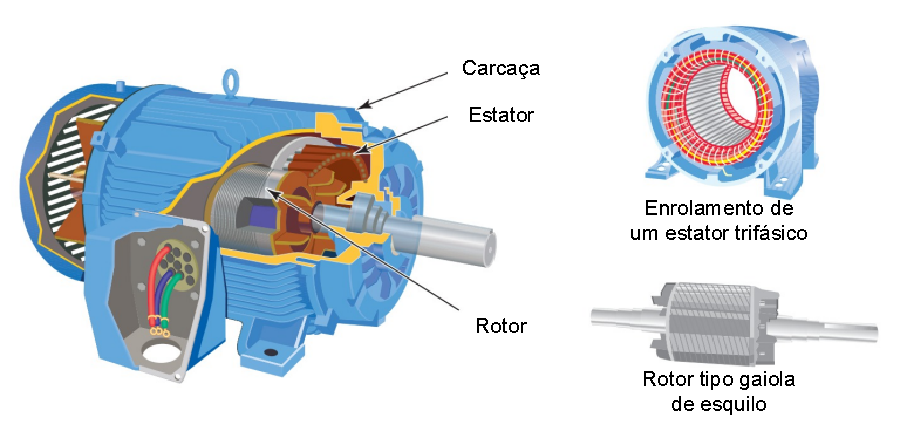
\includegraphics[scale=0.8, page=1]{referencial/img/imagens_referencial.pdf}
    \end{center}
    \fonte{Adaptado de \citeonline{Petruzella1911}.} 
    \label{fig:ind_motor_petruzella_p115}
\end{figure}

Uma das formas de se modelar um motor elétrico de indução, é através de uma representação em forma de um circuito 
elétrico, onde todas as variáveis podem ser representadas por componentes elétricos simples, facilitando a compreensão, modelagem e
prever possíveis variações nos elementos mecânicos e elétricos. O circuito representado na Figura \ref{fig:circuit_fitzgerald_p354},
é um circuito equivalente monofásico de um motor elétrico indutivo polifásico, o que simplifica toda a análise em um único circuito,
onde é trivial isolar a tensão em um terminal e a sua corrente. Para se saber as demais correntes e tensões, basta deslocar as fases
em $\pm\ang{120}$ \cite{Umans2003}.

\begin{figure}[H]
    \caption{Circuito equivalente monofásico de um motor de indução polifásico.}
    \begin{center}
        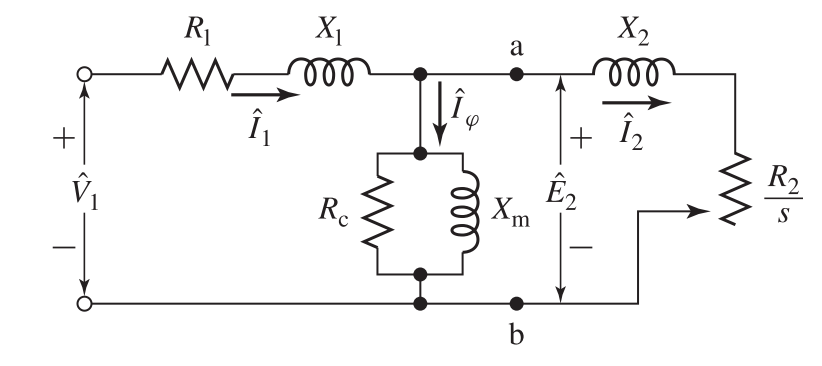
\includegraphics[scale=.35]{referencial/img/circuit_fitzgerald_p354.png}
    \end{center}
    \fonte{\citeonline{Umans2003}.} 
    \label{fig:circuit_fitzgerald_p354}
\end{figure}

Onde

\begin{itemize}
    \item $\hat{V}_1$ = tensão no estator
    \item $\hat{E}_2$ = Força eletromotriz contrária gerada pelo fluxo no entreferro
    \item $\hat{I}_1$ = corrente do estator
    \item $\hat{R}_1$ = resistência efetiva do estator
    \item $\hat{X}_1$ = reatância de vazamento do estator
    \item $R_c$ = resistência às perdas no núcleo
    \item $X_m$ = reatância magnetizante
    \item $\hat{I}_2$ = componente de corrente gerada pela carga
    \item $\hat{X}_2$ = reatância de vazamento do rotor no estator na frequência de escorregamento
    \item $R_2$ = resistência do rotor
    \item $\hat{I}_\varphi$ = componente de corrente excitada no estator
\end{itemize}

Com a apresentação de conceitos básicos sobre motores elétricos de indução e sua modelagem, é possível abordar os principais falhas que 
acometem as partes mecânicas e elétricas de um motor elétrico.


%----------------------------------------------------------------
% 
%----------------------------------------------------------------

\section{Falhas em Motores Elétricos de Indução}\label{sec:}

Como dito anteriormente, um motor elétrico é utilizado para transformar energia elétrica em mecânica, sendo empregado em máquinas que podem
realizar diversas atividades. A Figura \ref{fig:monitoring_methods_rilski_p78} representa uma generalização de um sistema em que um motor
elétrico é empregado. Nesta Figura, podemos ver os elementos que constituem a parte elétrica: a fonte de energia, o inversor de frequência e
o próprio motor. Também é possível ver a parte mecânica: a estrutura do motor, o acoplamento mecânico, a carga e as bases. Todos esses
elementos podem induzir falhas no motor, começando pelo acionamento, onde pode ocorrer uma falha e fazer o motor perder uma fase, ou ainda, 
oscilações na tensão e sobre carga. Todas essas falhas inevitavelmente alteram o espectro da fonte de energia \citeonline{Gorbounov2018}. 
Na parte mecânica, o desalinhamento entre a carga e o motor pode acarretar falhas no acoplamento que transfere a energia mecânica do motor
para o processo, e isso é normalmente provocado por uma instalação inapropriada.

\begin{figure}[H]
    \caption{Visão geral de sistema com um motor elétrico.}
    \begin{center}
        \includegraphics[scale=0.9, page=2]{referencial/img/imagens_referencial.pdf}
    \end{center}
    \fonte{Adaptado de \citeonline{Gorbounov2018}.} 
    \label{fig:motor_system_rilski_p2}
\end{figure}

A Figura \ref{fig:faults_rilski_p77} apresenta uma árvore das principais falhas que acometem os motores elétricos, sendo também divididas
em mecânicas e elétricas. 

\begin{figure}[H]
    \caption{Árvore dos principais tipos de falhas em motores elétricos.}
    \begin{center}
        \includegraphics[scale=1, page=3]{referencial/img/imagens_referencial.pdf}
    \end{center}
    \fonte{Adaptado de \citeonline{Gorbounov2018}.} 
    \label{fig:faults_rilski_p77}
\end{figure}

Dentre todas essas falhas, o trabalho aborda com maior foco as falhas mecânicas, mais especificamente desalinhamento, rolamentos 
e desbalanceamento que causam um aumento na vibração do sistema. O desalinhamento ocorre quando o motor e o sistema não estão perfeitamente alinhados, podendo ter dois tipos:
paralelo e angular, os quais podem ser vistos na Figura \ref{fig:misadraw_analog_p2}, respectivamente na parte (a) e (b) 
\cite{Sopcik2019}.

\begin{figure}[H]
    \caption{Ilustração com os tipos de desalinhamento.}
    \begin{center}
        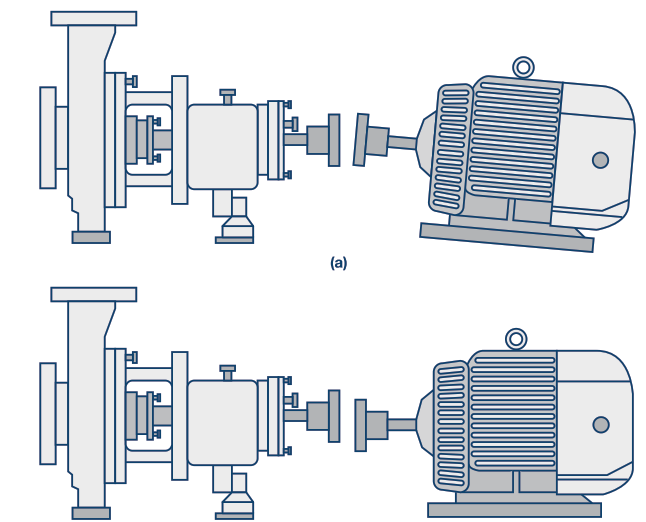
\includegraphics[scale=.35]{referencial/img/misadraw_analog_p2.png}
    \end{center}
    \fonte{\citeonline{Sopcik2019}.} 
    \label{fig:misadraw_analog_p2}
\end{figure}

Já a falha de desbalanceamento, pode ocorrer em qualquer parte rotativa do sistema, que vai desde o motor até a carga, compreendida por
algum problema na disposição das massas. Por último, os rolamentos, que são utilizados em diversas partes de um sistema e que podem
apresentar pequenas rachaduras na falta de lubrificação, que podem ser vistas na Figura \ref{fig:bearing_analog_p3}, aumentando a 
vibração \cite{Sopcik2019}.

\begin{figure}[H]
    \caption{Imagens de rolamentos no topo, e falhas na parte de baixo.}
    \begin{center}
        \includegraphics[scale=0.85, page=4]{referencial/img/imagens_referencial.pdf}
    \end{center}
    \fonte{Adaptado de \citeonline{Sopcik2019}.} 
    \label{fig:bearing_analog_p3}
\end{figure}

Mais de 66\% destas falhas são detectadas durante a operação e 28\% são encontradas apenas durante a manutenção 
preventiva \cite{Gorbounov2018}, destacando a importância de uma boa estratégia de manutenção. Existem três tipos de estratégias 
para manutenção \cite{Wu2013}:  

\begin{enumerate}
    \item Funcionar até quebrar: é uma das técnicas mais tradicionais, onde o equipamento funciona até quebrar. Só após isso a
manutenção é realizada. Possui diversas desvantagens, principalmente pelo fato que a falha pode se manifestar durante a produção e
deixar a máquina parada por horas, causando grande prejuízo;
    \item Manutenção Preventiva: é baseada em manutenções em intervalos regulares antes da falha se manifestar. Quando a frequência das
falhas é conhecida, pode ser uma boa estratégia, mas possibilita a troca de componentes que ainda teriam uma sobrevida, ou ainda, a falha
ocorrer antes do previsto, devido às alterações não esperada no processo;
    \item Manutenção Preditiva: quando é detectado que uma falha está próxima, antes de acontecer e com tempo ótimo para se fazer a 
manutenção sem afetar a produtividade e danificar mais o equipamento. Essa estratégia é baseada em um monitoramento do equipamento,
permitindo acompanhar o estado de saúde da máquina. Se bem implementa essa estratégia, pode reduzir em até 65\% os custos de manutenção
\cite{Wu2013};
\end{enumerate}

Após apresentados os conceitos básicos sobre motores elétricos e suas falhas, e como essas falhas aumentam o nível de vibração,
o próximo capítulo tem por objetivo apresentar conceitos de detecção e diagnóstico destas falhas.


%++++++++++++++++++++++++++++++++++++++++++++++++++++++++++++++++
% 
%++++++++++++++++++++++++++++++++++++++++++++++++++++++++++++++++

\section{Sistemas de Detecção e Diagnóstico de Falhas}\label{sec:}

Como apresentado anteriormente, falhas em componentes de um motor elétrico, ou no sistema em que ele está inserido, podem ocasionar
um aumento da vibração e alteração no espectro da corrente do motor, que serão estudados na sequência.


%----------------------------------------------------------------
% 
%----------------------------------------------------------------

\subsection{Análise de Vibração}\label{subsec:}

O aumento da vibração pode ocasionar perturbações até mesmo na parte elétrica de um motor, como mostra o gráfico que está na 
figura \ref{fig:fault_effect_randall_p54}. Com o aumento da carga e da vibração em conjunto, o efeito mecânico e elétrico pode ser 
severo \citeonline{Wu2013}.

\begin{figure}[H]
    \caption{Variação da carga para distinção da causa do efeito observado.}
    \begin{center}
        \includegraphics[scale=0.8, page=5]{referencial/img/imagens_referencial.pdf}
    \end{center}
    \fonte{Adaptado de \citeonline{Wu2013}.} 
    \label{fig:fault_effect_randall_p54}
\end{figure}


Essa vibração possui um característica específica, que depende de qual falha ela é oriunda, que acaba criando uma assinatura
ao se analisar a vibração, sendo possível diagnosticar se o motor e o sistema em que ele está inserido está com boa saúde \cite{Wu2013}.
Uma das primeiras técnicas para classificar o estado de saúde de uma máquina, é a norma ISO 10816-1, que recomenda níveis de vibração 
em valores eficaz de acordo com o porte da máquina, que pode ser visto na Tabela \ref{tab:iso10816-1_randall_p146}.

\begin{table}[H]
    \caption{Tabela de valores eficaz máximos de velocidade para cada porte de máquina indicados pela norma ISO 10816-1.}
    \label{tab:iso10816-1_randall_p146}
    \centering%
    \begin{minipage}{.9\textwidth}
        \begin{tabular*}{\textwidth}{|c|c|c|c|c|}
            \hline
            \multicolumn{1}{|c|}{Velocidade de vibração RMS [\SI{}{\milli\metre\per\second}] }& Classe I                                                         & Classe II                                                        & Classe III                                                       & Classe IV                                                        \\ \hline
            \multicolumn{1}{|c|}{0.25}            & \multicolumn{1}{c|}{\cellcolor[HTML]{00FF02}}                    & \multicolumn{1}{c|}{\cellcolor[HTML]{00FF02}}                    & \multicolumn{1}{c|}{\cellcolor[HTML]{00FF02}}                    & \multicolumn{1}{c|}{\cellcolor[HTML]{00FF02}}                    \\ \cline{1-1}
            \multicolumn{1}{|c|}{0.45}            & \multicolumn{1}{c|}{\cellcolor[HTML]{00FF02}}                    & \multicolumn{1}{c|}{\cellcolor[HTML]{00FF02}}                    & \multicolumn{1}{c|}{\cellcolor[HTML]{00FF02}}                    & \multicolumn{1}{c|}{\cellcolor[HTML]{00FF02}}                    \\ \cline{1-1}
            \multicolumn{1}{|c|}{0.71}            & \multicolumn{1}{c|}{\multirow{-3}{*}{\cellcolor[HTML]{00FF02}A}} & \multicolumn{1}{c|}{\cellcolor[HTML]{00FF02}}                    & \multicolumn{1}{c|}{\cellcolor[HTML]{00FF02}}                    & \multicolumn{1}{c|}{\cellcolor[HTML]{00FF02}}                    \\ \cline{1-2}
            \multicolumn{1}{|c|}{1.12}            & \multicolumn{1}{c|}{\cellcolor[HTML]{00D2CB}}                    & \multicolumn{1}{c|}{\multirow{-4}{*}{\cellcolor[HTML]{00FF02}A}} & \multicolumn{1}{c|}{\cellcolor[HTML]{00FF02}}                    & \multicolumn{1}{c|}{\cellcolor[HTML]{00FF02}}                    \\ \cline{1-1} \cline{3-3}
            \multicolumn{1}{|c|}{1.8}             & \multicolumn{1}{c|}{\multirow{-2}{*}{\cellcolor[HTML]{00D2CB}B}} & \multicolumn{1}{c|}{\cellcolor[HTML]{00D2CB}}                    & \multicolumn{1}{c|}{\multirow{-5}{*}{\cellcolor[HTML]{00FF02}A}} & \multicolumn{1}{c|}{\cellcolor[HTML]{00FF02}}                    \\ \cline{1-2} \cline{4-4}
            \multicolumn{1}{|c|}{2.8}             & \multicolumn{1}{c|}{\cellcolor[HTML]{F8FF00}}                    & \multicolumn{1}{c|}{\multirow{-2}{*}{\cellcolor[HTML]{00D2CB}B}} & \multicolumn{1}{c|}{\cellcolor[HTML]{00D2CB}}                    & \multicolumn{1}{c|}{\multirow{-6}{*}{\cellcolor[HTML]{00FF02}A}} \\ \cline{1-1} \cline{3-3} \cline{5-5} 
            \multicolumn{1}{|c|}{4.5}             & \multicolumn{1}{c|}{\multirow{-2}{*}{\cellcolor[HTML]{F8FF00}C}} & \multicolumn{1}{c|}{\cellcolor[HTML]{F8FF00}}                    & \multicolumn{1}{c|}{\multirow{-2}{*}{\cellcolor[HTML]{00D2CB}B}} & \multicolumn{1}{c|}{\cellcolor[HTML]{00D2CB}}                    \\ \cline{1-2} \cline{4-4}
            \multicolumn{1}{|c|}{7.1}             & \multicolumn{1}{c|}{\cellcolor[HTML]{FE0000}}                    & \multicolumn{1}{c|}{\multirow{-2}{*}{\cellcolor[HTML]{F8FF00}C}} & \multicolumn{1}{c|}{\cellcolor[HTML]{F8FF00}}                    & \multicolumn{1}{c|}{\multirow{-2}{*}{\cellcolor[HTML]{00D2CB}B}} \\ \cline{1-1} \cline{3-3} \cline{5-5} 
            \multicolumn{1}{|c|}{11.2}            & \multicolumn{1}{c|}{\cellcolor[HTML]{FE0000}}                    & \multicolumn{1}{c|}{\cellcolor[HTML]{FE0000}}                    & \multicolumn{1}{c|}{\multirow{-2}{*}{\cellcolor[HTML]{F8FF00}C}} & \multicolumn{1}{c|}{\cellcolor[HTML]{F8FF00}}                    \\ \cline{1-1} \cline{4-4}
            \multicolumn{1}{|c|}{18}              & \multicolumn{1}{c|}{\cellcolor[HTML]{FE0000}}                    & \multicolumn{1}{c|}{\cellcolor[HTML]{FE0000}}                    & \multicolumn{1}{c|}{\cellcolor[HTML]{FE0000}}                    & \multicolumn{1}{c|}{\multirow{-2}{*}{\cellcolor[HTML]{F8FF00}C}} \\ \cline{1-1} \cline{5-5} 
            \multicolumn{1}{|c|}{28}              & \multicolumn{1}{c|}{\cellcolor[HTML]{FE0000}}                    & \multicolumn{1}{c|}{\cellcolor[HTML]{FE0000}}                    & \multicolumn{1}{c|}{\cellcolor[HTML]{FE0000}}                    & \multicolumn{1}{c|}{\cellcolor[HTML]{FE0000}}                    \\ \cline{1-1} \cline{5-5} 
            \multicolumn{1}{|c|}{45}              & \multicolumn{1}{c|}{\multirow{-5}{*}{\cellcolor[HTML]{FE0000}D}} & \multicolumn{1}{c|}{\multirow{-4}{*}{\cellcolor[HTML]{FE0000}D}} & \multicolumn{1}{c|}{\multirow{-3}{*}{\cellcolor[HTML]{FE0000}D}} & \multicolumn{1}{c|}{\multirow{-2}{*}{\cellcolor[HTML]{FE0000}D}} \\ \cline{1-1} \cline{5-5}
        \end{tabular*}
      \fonte{Adaptado de \citeonline{Wu2013}.} 
    \end{minipage}
  \end{table}

Onde

\begin{itemize}
    \item A = bom estado
    \item B = aceitável
    \item C = apenas tolerável
    \item D = não permitido
    \item Classe I = pequenas máquinas (potência menor que $\SI{15}{\kilo\watt}$)
    \item Classe II = máquinas médias sem uma fundação especial (potência entre $\SI{15}{\kilo\watt}$ e $\SI{75}{\kilo\watt}$)
    \item Classe III = máquinas grandes sobre uma fundação rígida e pesada
    \item Classe IV = máquinas grandes sobre uma fundação flexível (turbomáquinas) 
\end{itemize}

Relembrando o que foi escrito anteriormente, é possível ver as assinaturas das falhas no espectro da vibração captada por um transdutor
que está acoplado no sistema. Quando uma falha de desalinhamento está presente, há um aumento de até duas vezes nas harmônicas de alta 
frequência, como pode ser visto na Figura \ref{fig:misa_analog_p2} \cite{Sopcik2019}.

\begin{figure}[H]
    \caption{Indicação espectral de desalinhamento na velocidade.}
    \begin{center}
        \includegraphics[scale=0.7, page=6]{referencial/img/imagens_referencial.pdf}
    \end{center}
    \fonte{Adaptado de \citeonline{Sopcik2019}.} 
    \label{fig:misa_analog_p2}
\end{figure}

Já quando uma falha de desbalanceamento está presente, há um aumento na harmônica principal da velocidade, em relação ao valor de base.
A Figura \ref{fig:imbalance_analog_p2} exemplifica.

\begin{figure}[H]
    \caption{Indicação espectral de desbalanceamento na velocidade.}
    \begin{center}
        \includegraphics[scale=0.8, page=7]{referencial/img/imagens_referencial.pdf}
    \end{center}
    \fonte{Adaptado de \citeonline{Sopcik2019}.} 
    \label{fig:imbalance_analog_p2}
\end{figure}

No mesmo conceito, é possível identificar a assinatura de uma falha de rolamentos de acordo com o tipo de rolamento, velocidade de rotação
do motor, entre outras características. Após a análise das falhas utilizando a vibração do sistema, é necessário fazer a mesma análise com a corrente elétrica na armadura, 
que será apresenta na subseção na sequência.



%++++++++++++++++++++++++++++++++++++++++++++++++++++++++++++++++
% 
%++++++++++++++++++++++++++++++++++++++++++++++++++++++++++++++++

\section{Técnicas de Processamento de Sinais}\label{sec:signal_process}

Com o objetivo de se detectar falhas e se obter um diagnóstico das mesmas, muitas técnicas já foram implementadas. Essas técnicas podem ser
não invasivas ou invasivas \cite{Gorbounov2018}. A Figura \ref{fig:monitoring_methods_rilski_p78} apresenta algumas técnicas que são
utilizadas para detecção e diagnóstico de falhas.

\begin{figure}[H]
    \caption{Árvore de métodos de monitoramento de falhas em motores elétricos.}
    \begin{center}
        \includegraphics[scale=0.9, page=8]{referencial/img/imagens_referencial.pdf}
    \end{center}
    \fonte{Adaptado de \citeonline{Gorbounov2018}.} 
    \label{fig:monitoring_methods_rilski_p78}
\end{figure}

Dentre estas, a FFT (\textit{Fast Fourier Transform - transformada rápida de Fourier}), Valor RMS (\textit{Root Mean Square} - valor quadrático 
médio) e ML \textit{machine learning} (aprendizado de máquina) serão utilizadas de forma direta ou indireta neste trabalho.
FFT é um algoritmo muito eficiente que calcula a DFT (\textit{Discrete Fourier Transform} - Transformada  discreta de Fourier), a qual pode ser
descrita da seguinte forma \cite{Wu2013}:

\begin{equation}\label{eq:dft}
    G(k)=\frac{1}{N}\sum_{k=0}^{N-1} g(n)exp(-j2\pi kn/N)
\end{equation}

\begin{equation}\label{eq:dft2}
    g(n)=\sum_{k=0}^{N-1} G(k)exp(j2\pi kn/N)
\end{equation}

Esta ferramenta é utilizada para se se representar no domínio da frequência, sinais discretos que estão no domínio do tempo. Isto 
possibilita extrair informações do espectro desses sinais, conforme descrito na seção anterior. 

Já o Valor RMS, que é a representação mais comum de se descrever a energia que um sinal  $x(t)$ carrega em qualquer período \cite{Cryer2010}, 
que pode ser representado da seguinte forma:

\begin{equation}\label{eq:rms_int}
    X_{RMS} = \sqrt{\frac{1}{T}\int_{0}^{T}{x(t)^2dt}}
\end{equation}

A ideia de se caracterizar a energia de um sinal através do Valor RMS \cite{Cryer2010}, vem da seguinte expressão:

\begin{equation}\label{eq:energia}
    E = \int_{0}^{T}{[x(t)]^2dt}
\end{equation}

Onde $E$ é a energia carregada pelo sinal x(t) \cite{Oppenheim2016}. Expandindo, se calcularmos a potência dissipada em um resistor de
$\SI{1}{\ohm}$ num intervalo de tempo T, temos a seguinte expressão:

\begin{equation}\label{eq:power}
    P = \frac{1}{T}\int_{0}^{T}{[x(t)]^2dt}
\end{equation}

Se compararmos as equações \ref{eq:rms_int} e \ref{eq:power}, vemos que o valor RMS está relacionado com a raiz quadrada da potência do 
sinal. Ao se utilizar sinais discretos, o valor RMS pode ser representado da seguinte forma:

\begin{equation}\label{eq:rms_disc}
    x_{RMS} = \sqrt{\frac{1}{N}\sum_{i=1}^{N}{X^2(i)}}
\end{equation}

A última das técnicas utilizadas neste trabalho, ML, que nasceu dentro da ciência da computação, e que veio ao encontro do reconhecimento de 
padrões, já este, oriundo das engenharias, para formar uma ferramenta importantíssima para as ciências, com as mais diversas
aplicações. No campo do reconhecimento de padrões, a palavra-chave é a incerteza. Teoria da probabilidade é uma ferramenta matemática sólida
para quantificar e manipular incertezas, formando a fundamentação para o recondicionamento de padrões. O estudo da 
distribuição de probabilidades em variáveis contínuas é essencial para entender a dinâmica destes dados. A distribuição de probabilidades mais
conhecida é a Gaussiana, que também é chamada de distribuição normal \cite{Andersen1986}. Três dos principais parâmetros para se analisar
em uma distribuição normal são: média, variância e desvio padrão, onde a média de um sinal $x(t)$ num período T, pode ser calculado da seguinte
forma \cite{Dinardo}:

\begin{equation}\label{eq:X_lim}
    \bar{x} = \lim_{T\rightarrow\infty}{\frac{1}{T^*}} \int_{0}^{T}{x(t)dt}
\end{equation}

Já a variância:

\begin{equation}\label{eq:variancia}
    \sigma^2 = \lim_{T^{*}\rightarrow\infty}{\frac{1}{T^*}} \int_{0}^{T}{[x(t)-\bar{x}]^2dt}
\end{equation}

Onde $\sigma$ é o desvio padrão, que representa a dispersão, em outras palavras, o quão distante os dados amostrados estão da média. Um dado
amostrado que se encontra disperso, ou seja, com elevado desvio padrão, pode significar que houve um ganho ou perda de energia, se esse dado
for um valor RMS, caracterizando uma anomalia. Assim que os conceitos básicos foram apresentados, podemos relacionar os trabalhos correlatos,
os quais serão descritos na próxima etapa.


%++++++++++++++++++++++++++++++++++++++++++++++++++++++++++++++++
% 
%++++++++++++++++++++++++++++++++++++++++++++++++++++++++++++++++

\section{Estado da Arte}

O estado da arte em detecção e diagnóstico de falhas em motores elétricos está no emprego de diversas técnicas numa mesma solução. Algumas 
utilizam técnicas clássicas, outras empregam diversas técnicas modernas para se obter o resultado ótimo. A presente seção contém
alguns exemplos que empregam novos arranjos de técnicas, as quais já foram discutidas anteriormente. 

A busca pela compreensão dos padrões das falhas em máquinas rotativas e não rotativas, com o foco na análise dos níveis de vibração. O artigo
\cite{Jeong2016} busca encontrar e entender estes padrões em orbitais gerados pela vibração conjugada entre dois eixos, o axial e o radial. A
vibração é tratada no plano complexo, e imagens são geradas a partir desta representação e classificadas por uma 
CNN (\textit{Convolutional Neural network} - rede neural convolucional), que apresentou erro de \SI{1.3}{\percent} na classificação das falhas.
Este foi o primeiro trabalho estudado, influenciando  diretamente os primeiros meses do desenvolvimento do presente trabalho, onde a busca se
deu pela detecção e classificação das falhas.

Outra forma de detecção de falhas e diagnóstico utilizando rede neural convolucional, é através do processamento dos sinais de corrente. O 
artigo \cite{Ince2016} trata deste tema ao utilizar uma CNN unidimensional para classificar as falhas. Como o método anterior, o treinamento
ocorre de forma \textit{offline}, além de tratar os sinais de corrente, que possuem limitações na amostragem e na construção dos sensores, que
precisam ser não invasivos e não influenciáveis pelos inversores de frequência, encarecendo o hardware, ou até limitando o uso. Os
resultados foram bem satisfatórios, com acurácia de mais de \SI{97}{\percent}, com tempo de processamento inferior a \SI{450}{\milli\second}.

Outra técnica aplicada na detecção e diagnóstico de falhas, é a transformada Wavelet, conforme a figura \ref{fig:monitoring_methods_rilski_p78}.
O artigo \cite{Hemmati2016a} trata deste assunto. No artigo, características de um sinal de vibração são levantadas e comparadas,
onde uma delas é o estudo do valor RMS, tratado anteriormente na etapa de conceitos básicos. Uma das principais conclusões do trabalho, é que o 
valor RMS é o melhor parâmetro estatístico para detectar uma falha incipiente.

Contribuindo com a tendência ao processamento de imagens para a detecção e diagnóstico de falhas, o artigo \cite{Hatami2017} trata deste tema
utilizando CNN, mas com a transformação das séries temporais em imagens em duas dimensões e após isso, aplicadas em uma CNN. Estas imagens são
texturizadas de acordo com as características dos sinais. Este trabalho também apresentou resultado satisfatório.

Outro trabalho importante \cite{Caesarendra2017} , é o qual realizou uma pesquisa sistemática com as principais técnicas de detecção de 
falhas que são estatísticas. Neste trabalho foram analisadas ferramentas como Kurtosis, Variância e valor RMS. As técnicas foram aplicadas em 
dados gerados em laboratório, e resultados foram elencados. Levanta a questão que o valor RMS é relevante para detectar iminentes falhas, mas
limitado para se diagnosticar falhas.

A técnica ICA (\textit{Indepent Compoent Analysys}- análise de componentes independentes) também está muito presente nos trabalhos atuais. O 
artigo \cite{Garcia-Bracamonte2019} utiliza essa técnica combinada com uma rede neural artificial para fazer a detecção e diagnóstico, 
nesta ordem, utilizando sinais de corrente. O trabalho é muito rico de análise estatística, com resultados satisfatórios, tendo
um protótipo e um estudo de caso do método desenvolvido.

O uso da ferramenta FFT pura também foi listado durante as pesquisas. O artigo \cite{Azeem2019} a utiliza para detectar desalinhamento, e o
estudo experimental aconteceu com o uso do mesmo modelo de simulador de falhas que foi utilizado neste trabalho, que será explicado no próximo
capítulo. Ao analisar o espectro e levantar as assinaturas, os resultados deste trabalho também se mostraram satisfatórios. 

Outro exemplo de trabalho importante, mesmo que não se tratando da análise de vibração de motores, e sim de transformadores, é o artigo \cite{Zhang2019}.
Ele apresenta um software para monitorar em tempo real a vibração de transformadores, utilizando algumas ferramentas estatísticas e transformada
Wavelet. Utilizou o software labview para a implementação da metodologia desenvolvida, obtendo os resultados esperados. A tabela
\ref{tab:correlatos} relaciona todos os trabalhos anteriormente discutidos.

\begin{table}[H]
    \caption{Tabela de trabalhos correlatos.}
    \label{tab:correlatos}
    \centering%
        \begin{tabular}{|p{0.06\textwidth}|p{0.2\textwidth}|p{0.32\textwidth}|p{0.32\textwidth}|}
            \hline
            Ano  & Autores                      & Trabalho Realizado                                                                    & Relação                        \\ \hline
            2016 & \cite{Jeong2016}             & Detecção e classificação de falhas pela geração de orbitais                           & Motivação inicial e emprego de ML \\ \hline
            2016 & \cite{Ince2016}              & Detecção de falhas através da análise da corrente elétrica via CNN                    & Estudo da viabilidade do uso da corrente elétrica \\ \hline
            2016 & \cite{Hemmati2016a}          & Estração de assinaturas via transformada Wavelet                                      & Estudo do valor RMS na detecção de falhas \\ \hline
            2017 & \cite{Hatami2017}            & Criação de imagens 2D texturizadas e classificadas via CNN                            & Alternativa para análise de falhas em sinais de vibração \\ \hline
            2017 & \cite{Caesarendra2017}       & Revisão sistemática de ferramentas estatísticas para detecção e diagnóstico de falhas & Valor RMS \\ \hline
            2019 & \cite{Garcia-Bracamonte2019} & Emprego de ICA para detecção e diagnóstico através de sinais de corrente.             & Estudo estatístico e criação de um protótipo \\ \hline
            2019 & \cite{Azeem2019}             & Emprego da FFT                                                                        & FFT e simulador de falhas \\ \hline
            2019 & \cite{Zhang2019}             & Sistema para monitoramento em tempo real utilizando ferramentas estatísticas          & Ferramentas estatísticas e software para monitoramento em tempo real \\ \hline        
        \end{tabular}
      \fonte{Elaborado pelo autor.} 
  \end{table}

Concluída a apresentação de alguns trabalhos que contém alguma relação com o presente trabalho, onde características importantes e resultados 
foram apresentados, podemos prosseguir para o próximo capítulo, etapa esta em que a proposta do atual trabalho é apresentada e implementada.